\documentclass{beamer} 
\usepackage{amsmath,amsthm}
\usepackage{graphicx,microtype,parskip}
\usepackage{caption,subcaption,multirow}
\usepackage{attrib}

\frenchspacing

\usetheme{default}
\usecolortheme{whale}

\setbeamertemplate{navigation symbols}{}

\setbeamercolor{title}{fg=blue,bg=white}

\setbeamercolor{block title}{fg=white,bg=gray}
\setbeamercolor{block body}{fg=black,bg=lightgray}

\setbeamercolor{block title alerted}{fg=white,bg=darkgray}
\setbeamercolor{block body alerted}{fg=black,bg=lightgray}

\title{How do species traits affect extinction risk?}
\subtitle{New approaches to old questions.}
\author{Peter D Smits}
\institute{Committee on Evolutionary Biology}
\titlegraphic{
  
\includegraphics[width=2.75cm,height=2.75cm,keepaspectratio=true]{figure/paleodb}
  \hspace*{0.35\paperwidth}
  
\includegraphics[width=2cm,height=2cm,keepaspectratio=true]{figure/chicago}
}
\date{}

\begin{document}

\begin{frame}
  \titlepage
\end{frame}

\begin{frame}
  \begin{alertblock}{Question}
    Why do taxa go extinct at different rates?
  \end{alertblock}
\end{frame}

\begin{frame}
  \frametitle{Two studies}

  \begin{columns}
    \begin{column}{0.5\textwidth}
      \begin{center}
        \textbf{Mammals}

        \vspace{0.5cm}

        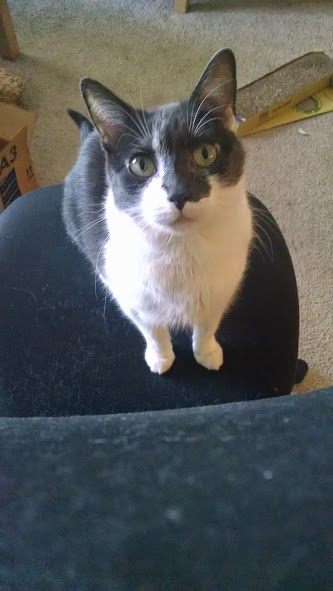
\includegraphics[height = 0.555\textheight, keepaspectratio = true]{figure/annyong_2}
      \end{center}
    \end{column}
    \begin{column}{0.5\textwidth}
      \begin{center}
        \textbf{Brachiopods}
        
        \vspace{0.63cm}

        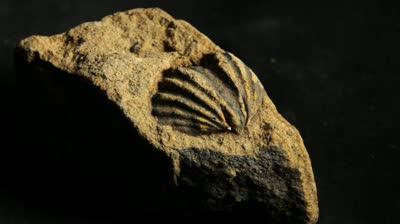
\includegraphics[height = 0.25\textheight, keepaspectratio = true]{figure/stock-brac2}
        
        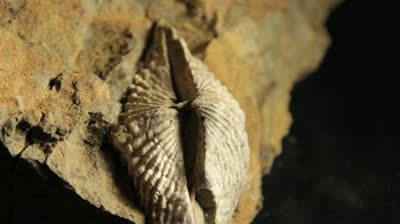
\includegraphics[height = 0.25\textheight, keepaspectratio = true]{figure/stock-brac3}
        
        \tiny{\attrib{Immersion Imagery, Shutterstock}}
      \end{center}
    \end{column}
  \end{columns}
\end{frame}

\begin{frame}
  \frametitle{Hierarchical Bayesian modeling}

  
\includegraphics[width = \textwidth,height = 0.8\textheight,keepaspectratio = true]{figure/han_bayes}

  \tiny{\attrib{www.countbayesie.com}}
\end{frame}

\begin{frame}
  \frametitle{First things first\dots}

  \begin{block}{(Some) notational definitions to help navigate}
    \begin{itemize}
      \item \(y_{i}\): duration of taxon \(i\)
      \item \(\mathbf{X}\): \(n \times k\) matrix of covariates
      \item \(\sim\): rhs stochastically distributed as lhs
      \item \(\beta\): regression coefficient (covariate effect)
      \item \(j[i]\): taxon \(i\) belongs to group \(j\)
    \end{itemize}
  \end{block}
\end{frame}

\begin{frame}
  \frametitle{Study: mammal species duration}

  \begin{alertblock}{Questions}
    \begin{itemize}
      \item How do the covariates of interest affect extinction risk?
        \begin{itemize}
          \item dietary and locomotor category, \\bioprovince occupancy, body size
        \end{itemize}
      \item What is the relative contribution of temporal and phylogenetic structure on extinction risk?
      \item How do the identified time-invariant effects compare to modern determinates of extinction risk?
    \end{itemize}
  \end{alertblock}
\end{frame}

\begin{frame}
  \frametitle{Model of mammal species survival}

  \begin{columns}
    \begin{column}{0.5\textwidth}
      % need to cut the white space from this image
      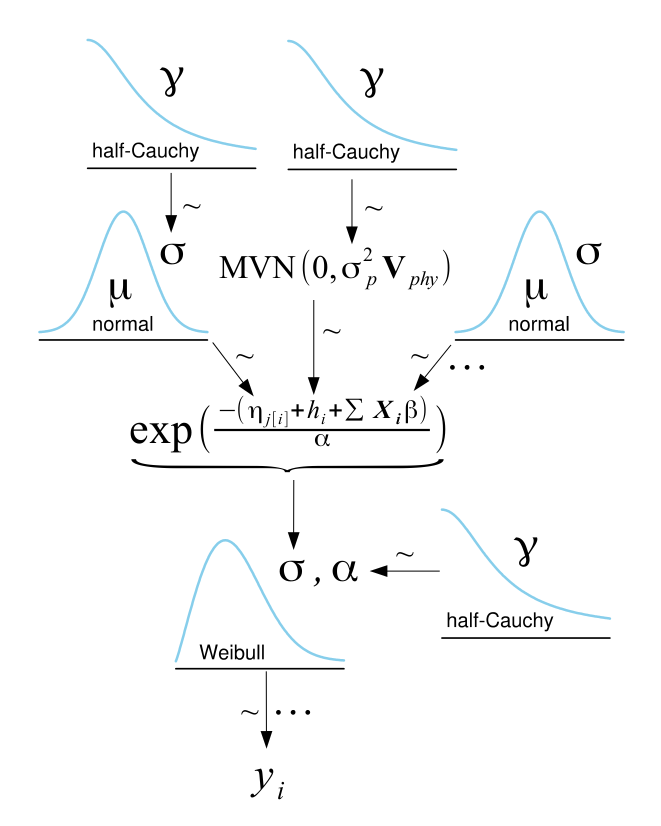
\includegraphics[width=\textwidth,keepaspectratio=true]{figure/mammal_model}
    \end{column}
    \begin{column}{0.5\textwidth}
      non-nested varying intercept
      \begin{itemize}
        \item origination cohort (\(\eta_{j[i]} \text{ for } j = 1,\dots,J\))
          \begin{itemize}
            \item exchangable; \(\mathcal{N}(0, \sigma_{\eta})\)
          \end{itemize}
        \item phylogenetic position (\(h_{i} \text{ for } i = 1,\dots,N\))
          \begin{itemize}
            \item supertree \\(mostly taxonomy)
            \item mbl scaling; \\resolved based on FAD
            \item Brownian motion
          \end{itemize}
      \end{itemize}
    \end{column}
  \end{columns}
\end{frame}


\begin{frame}
  \frametitle{Results}
  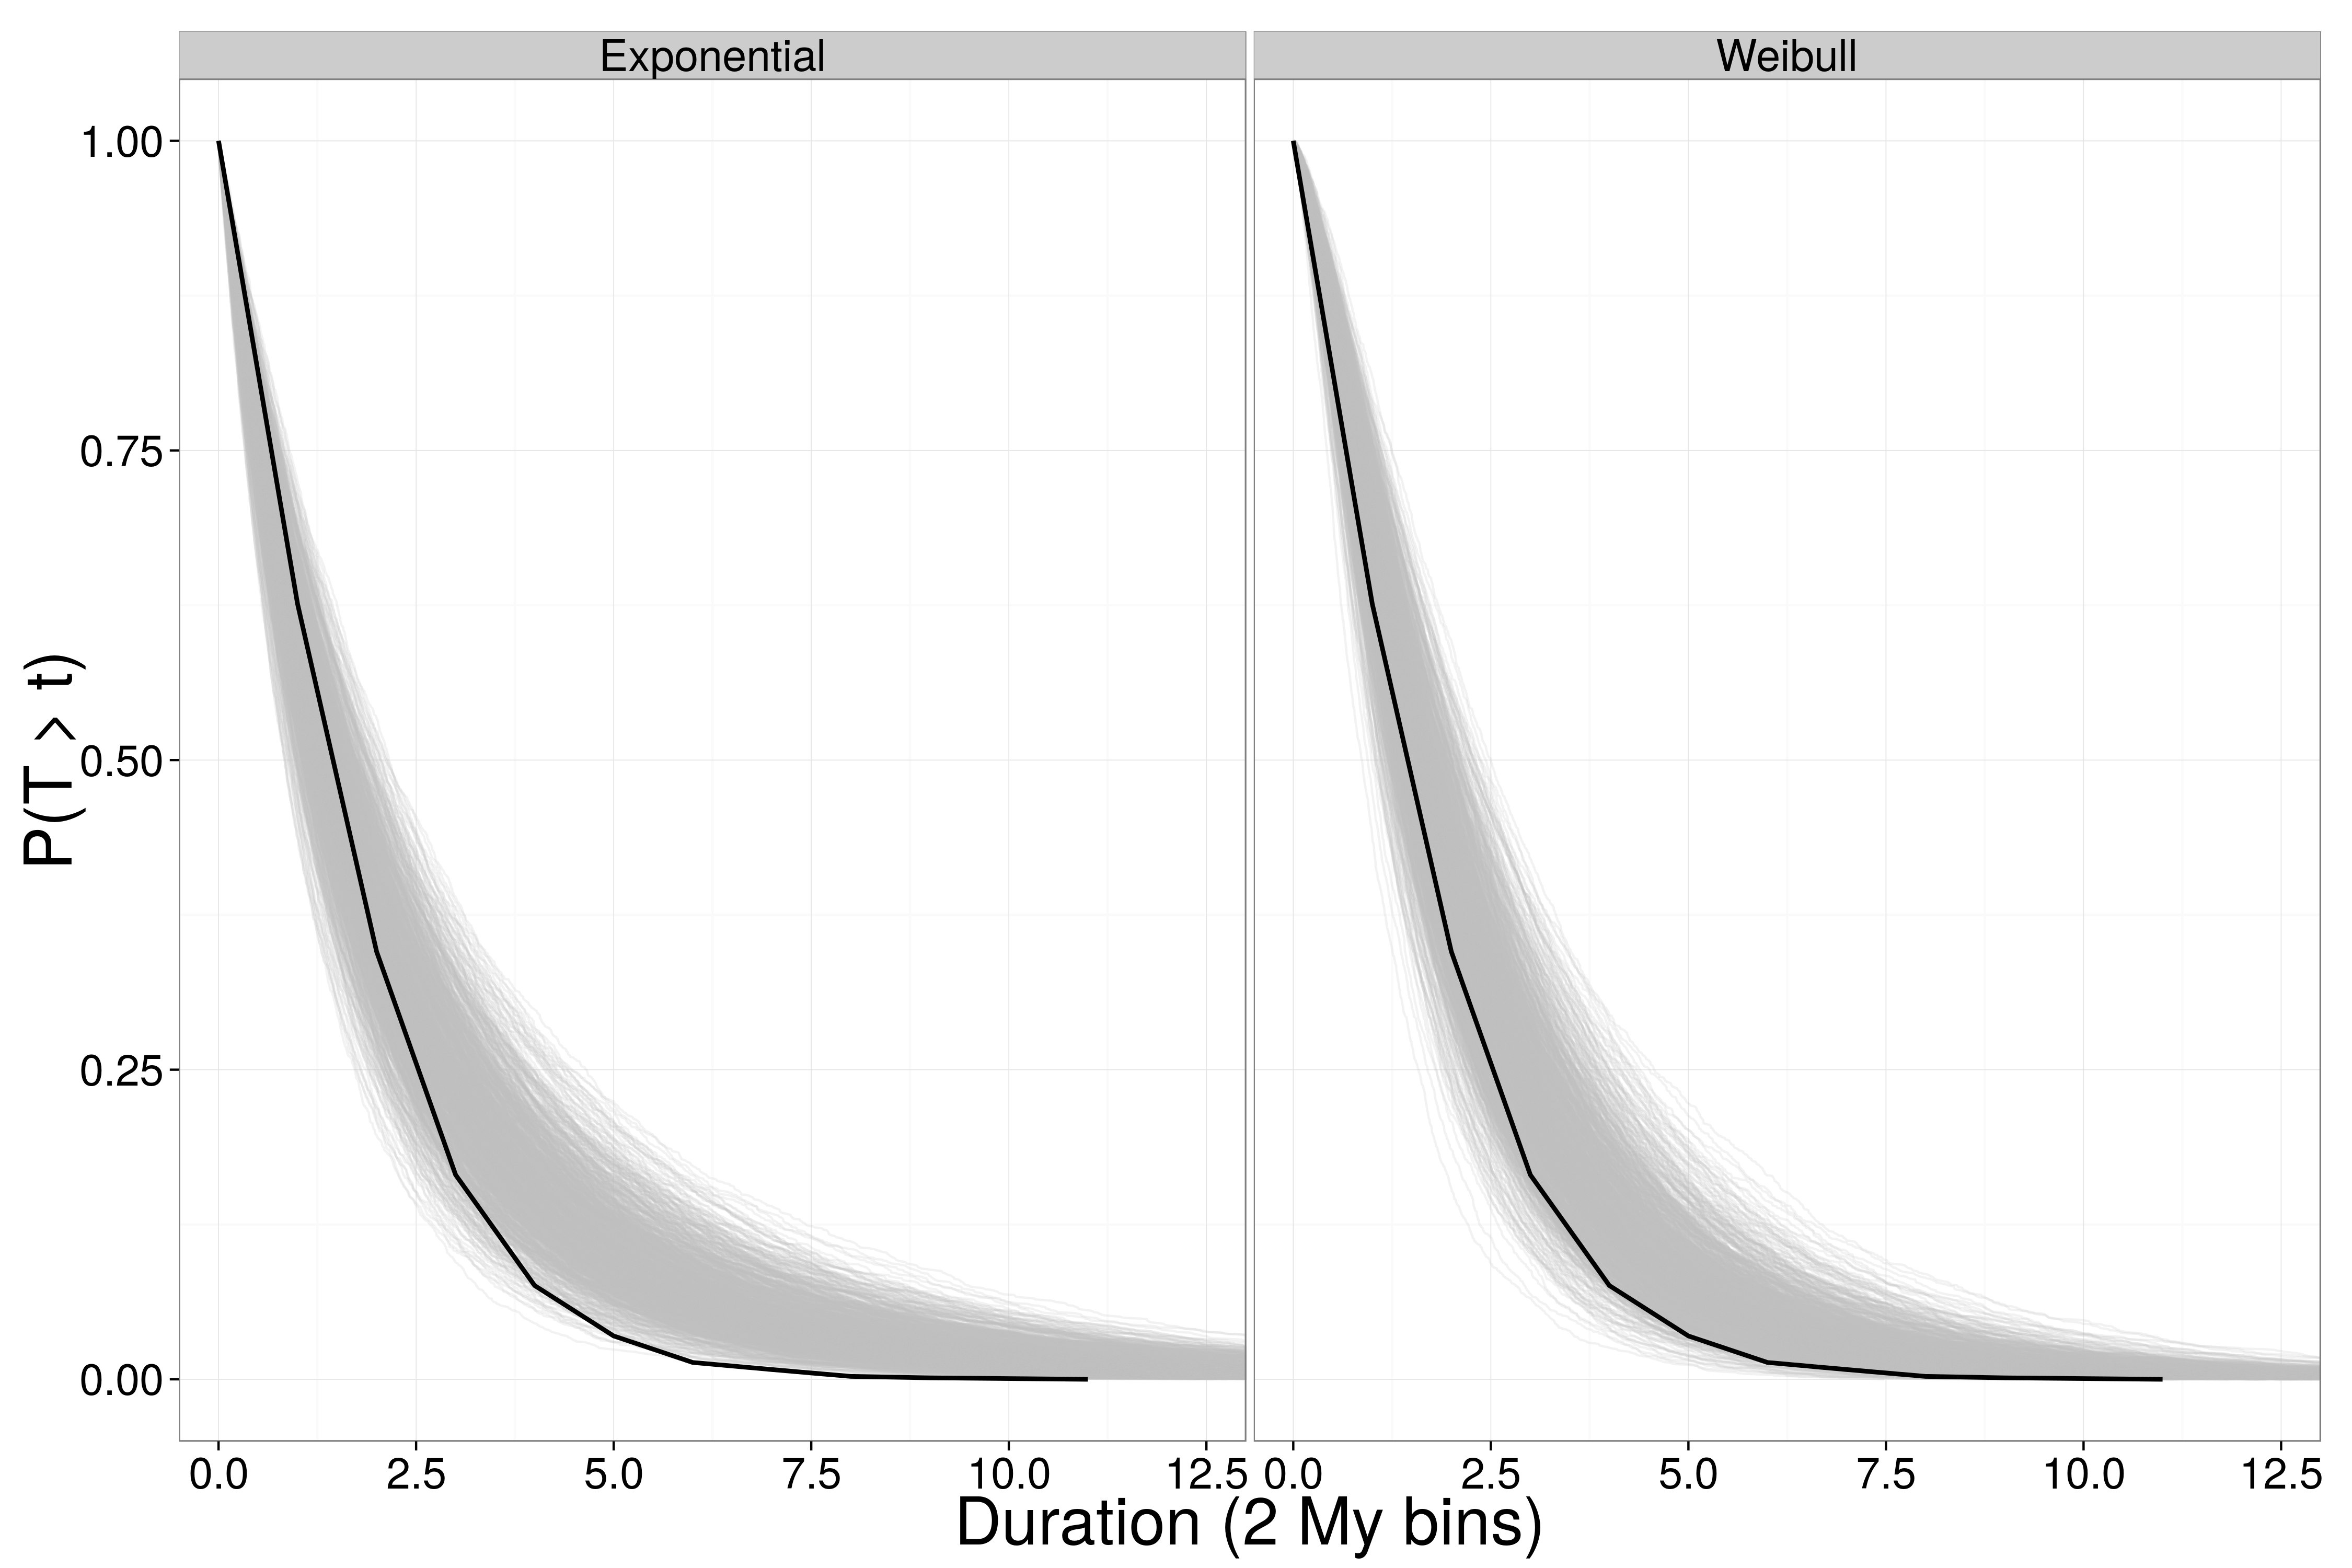
\includegraphics[width=\textwidth,height=0.8\textheight,keepaspectratio=true]{figure/survival_function}
  
  \tiny{\attrib{Smits, \textit{Submitted}}}
\end{frame}

\begin{frame}
  \frametitle{Results}
  \begin{columns}
    \begin{column}{0.5\textwidth}
      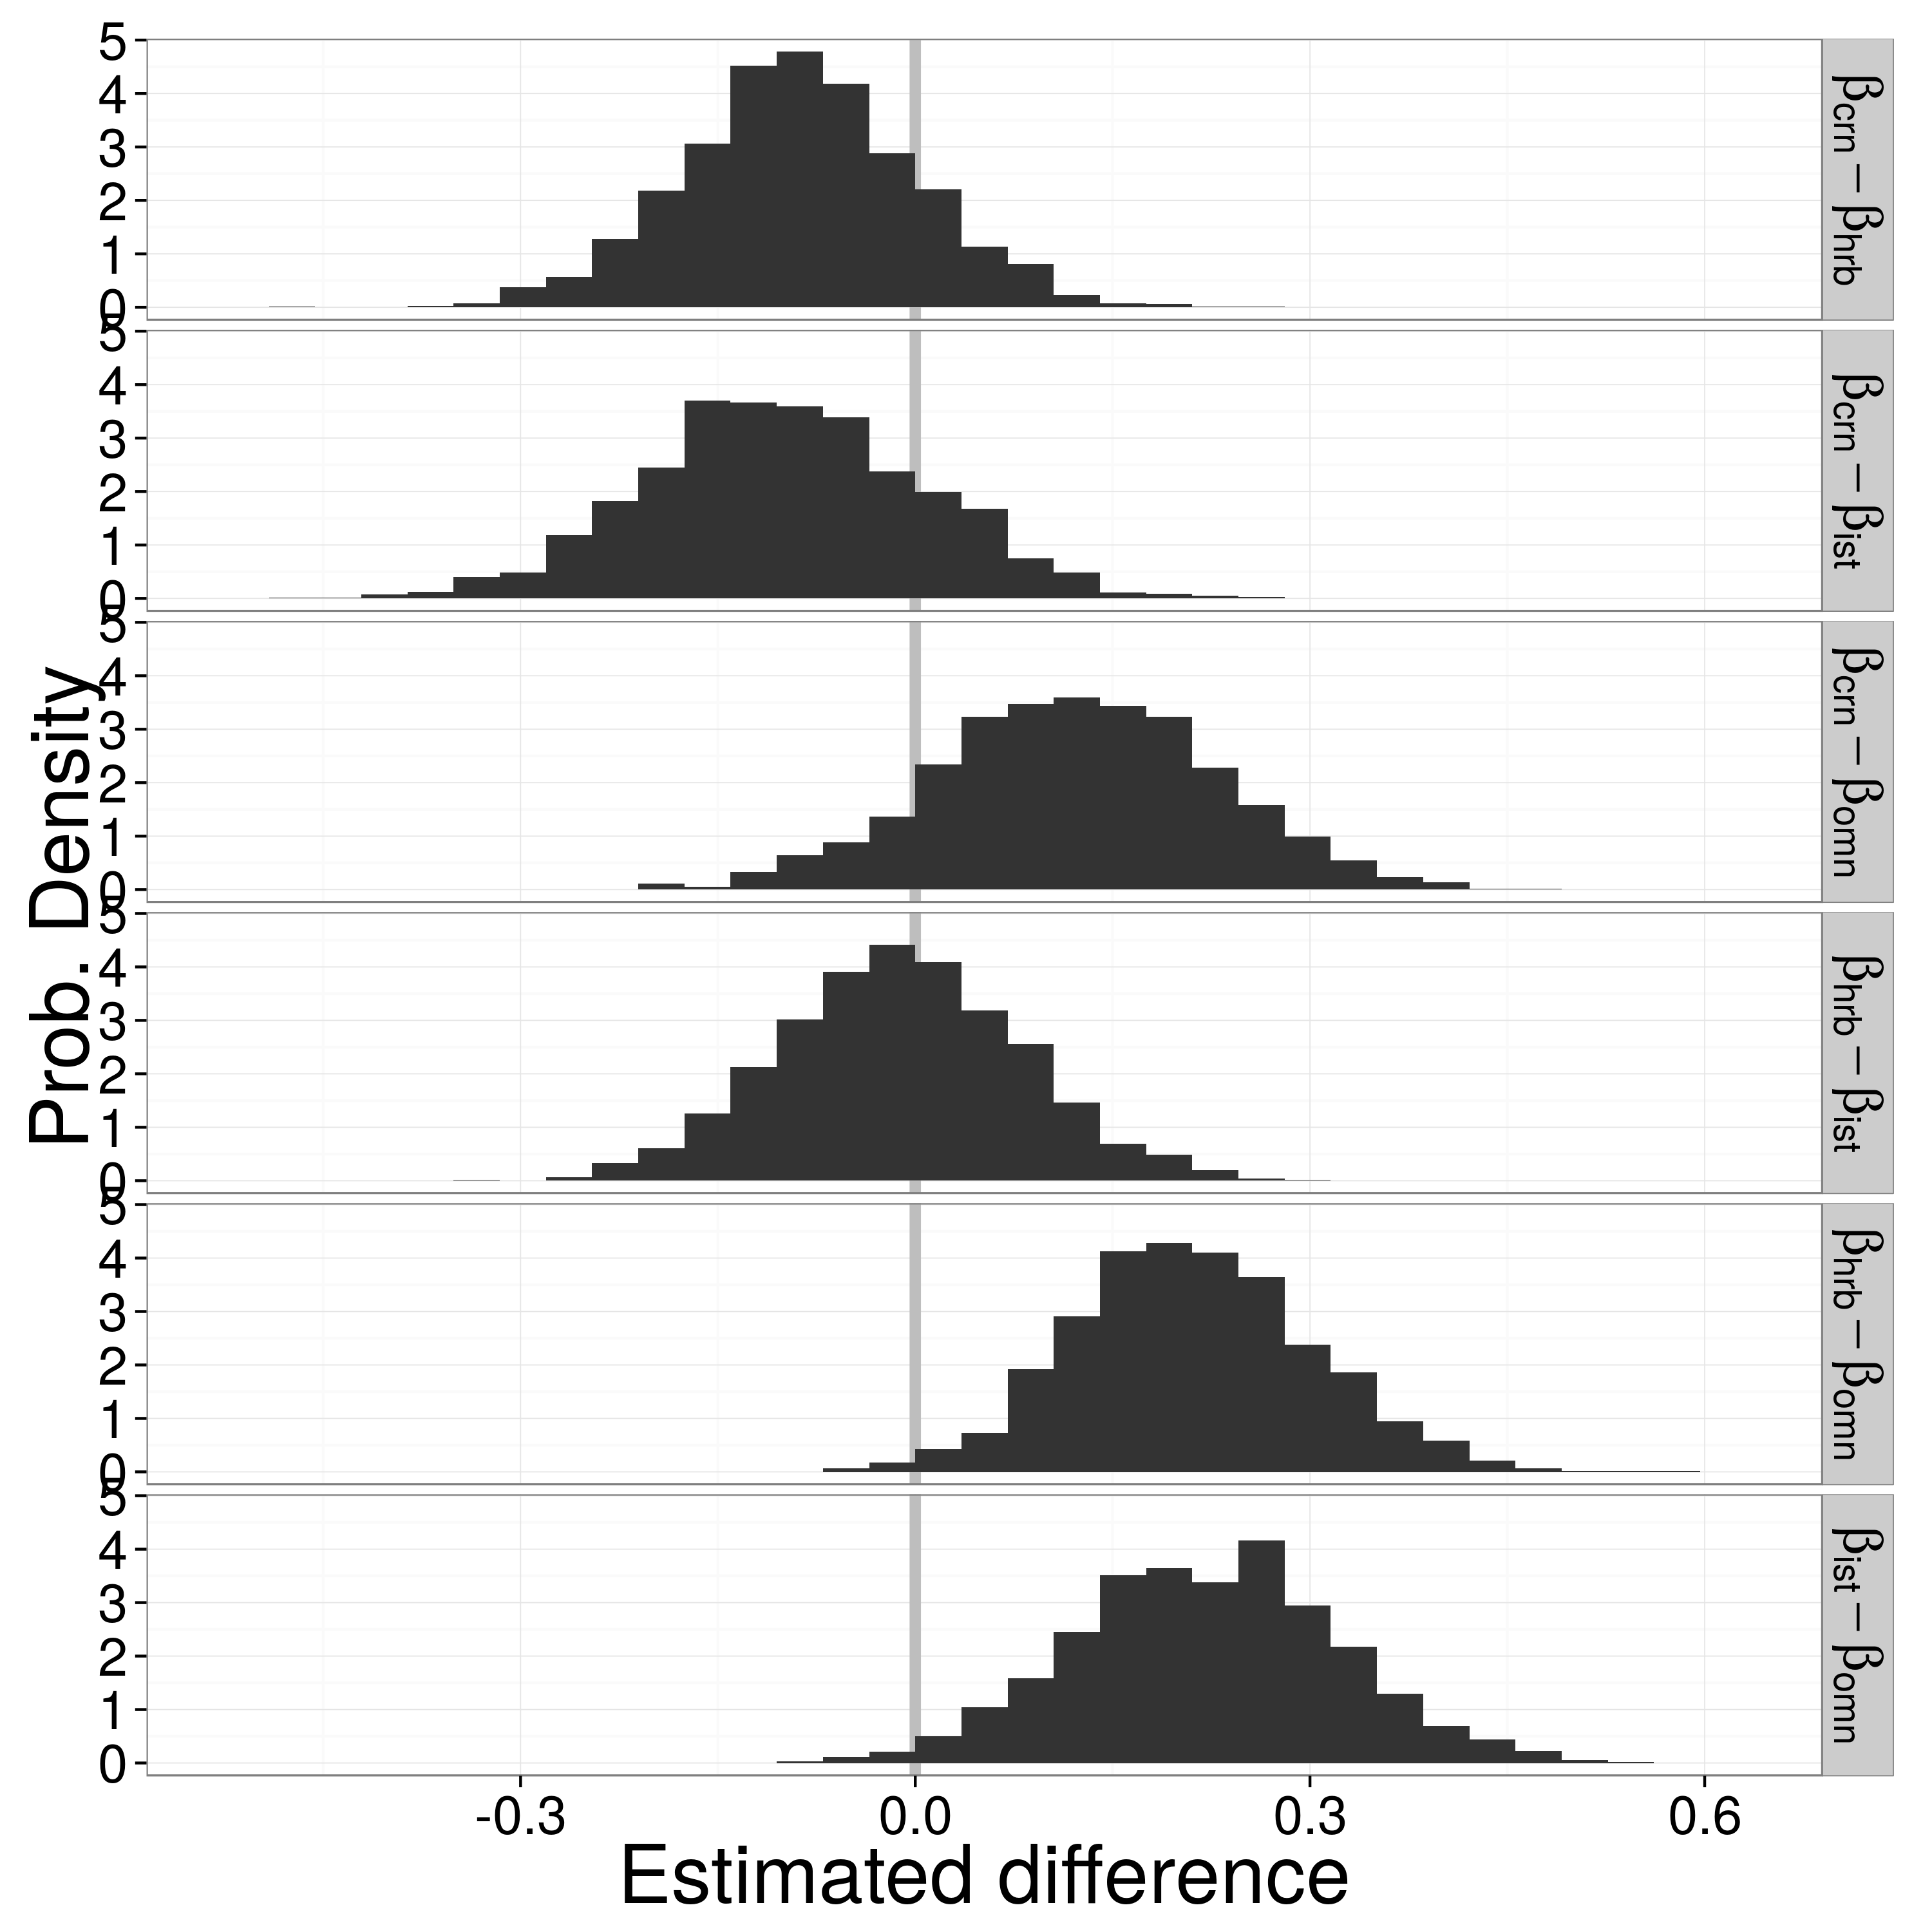
\includegraphics[width=\textwidth,height=0.8\textheight,keepaspectratio=true]{figure/diet_diff_est}
    \end{column}
    \begin{column}{0.5\textwidth}
      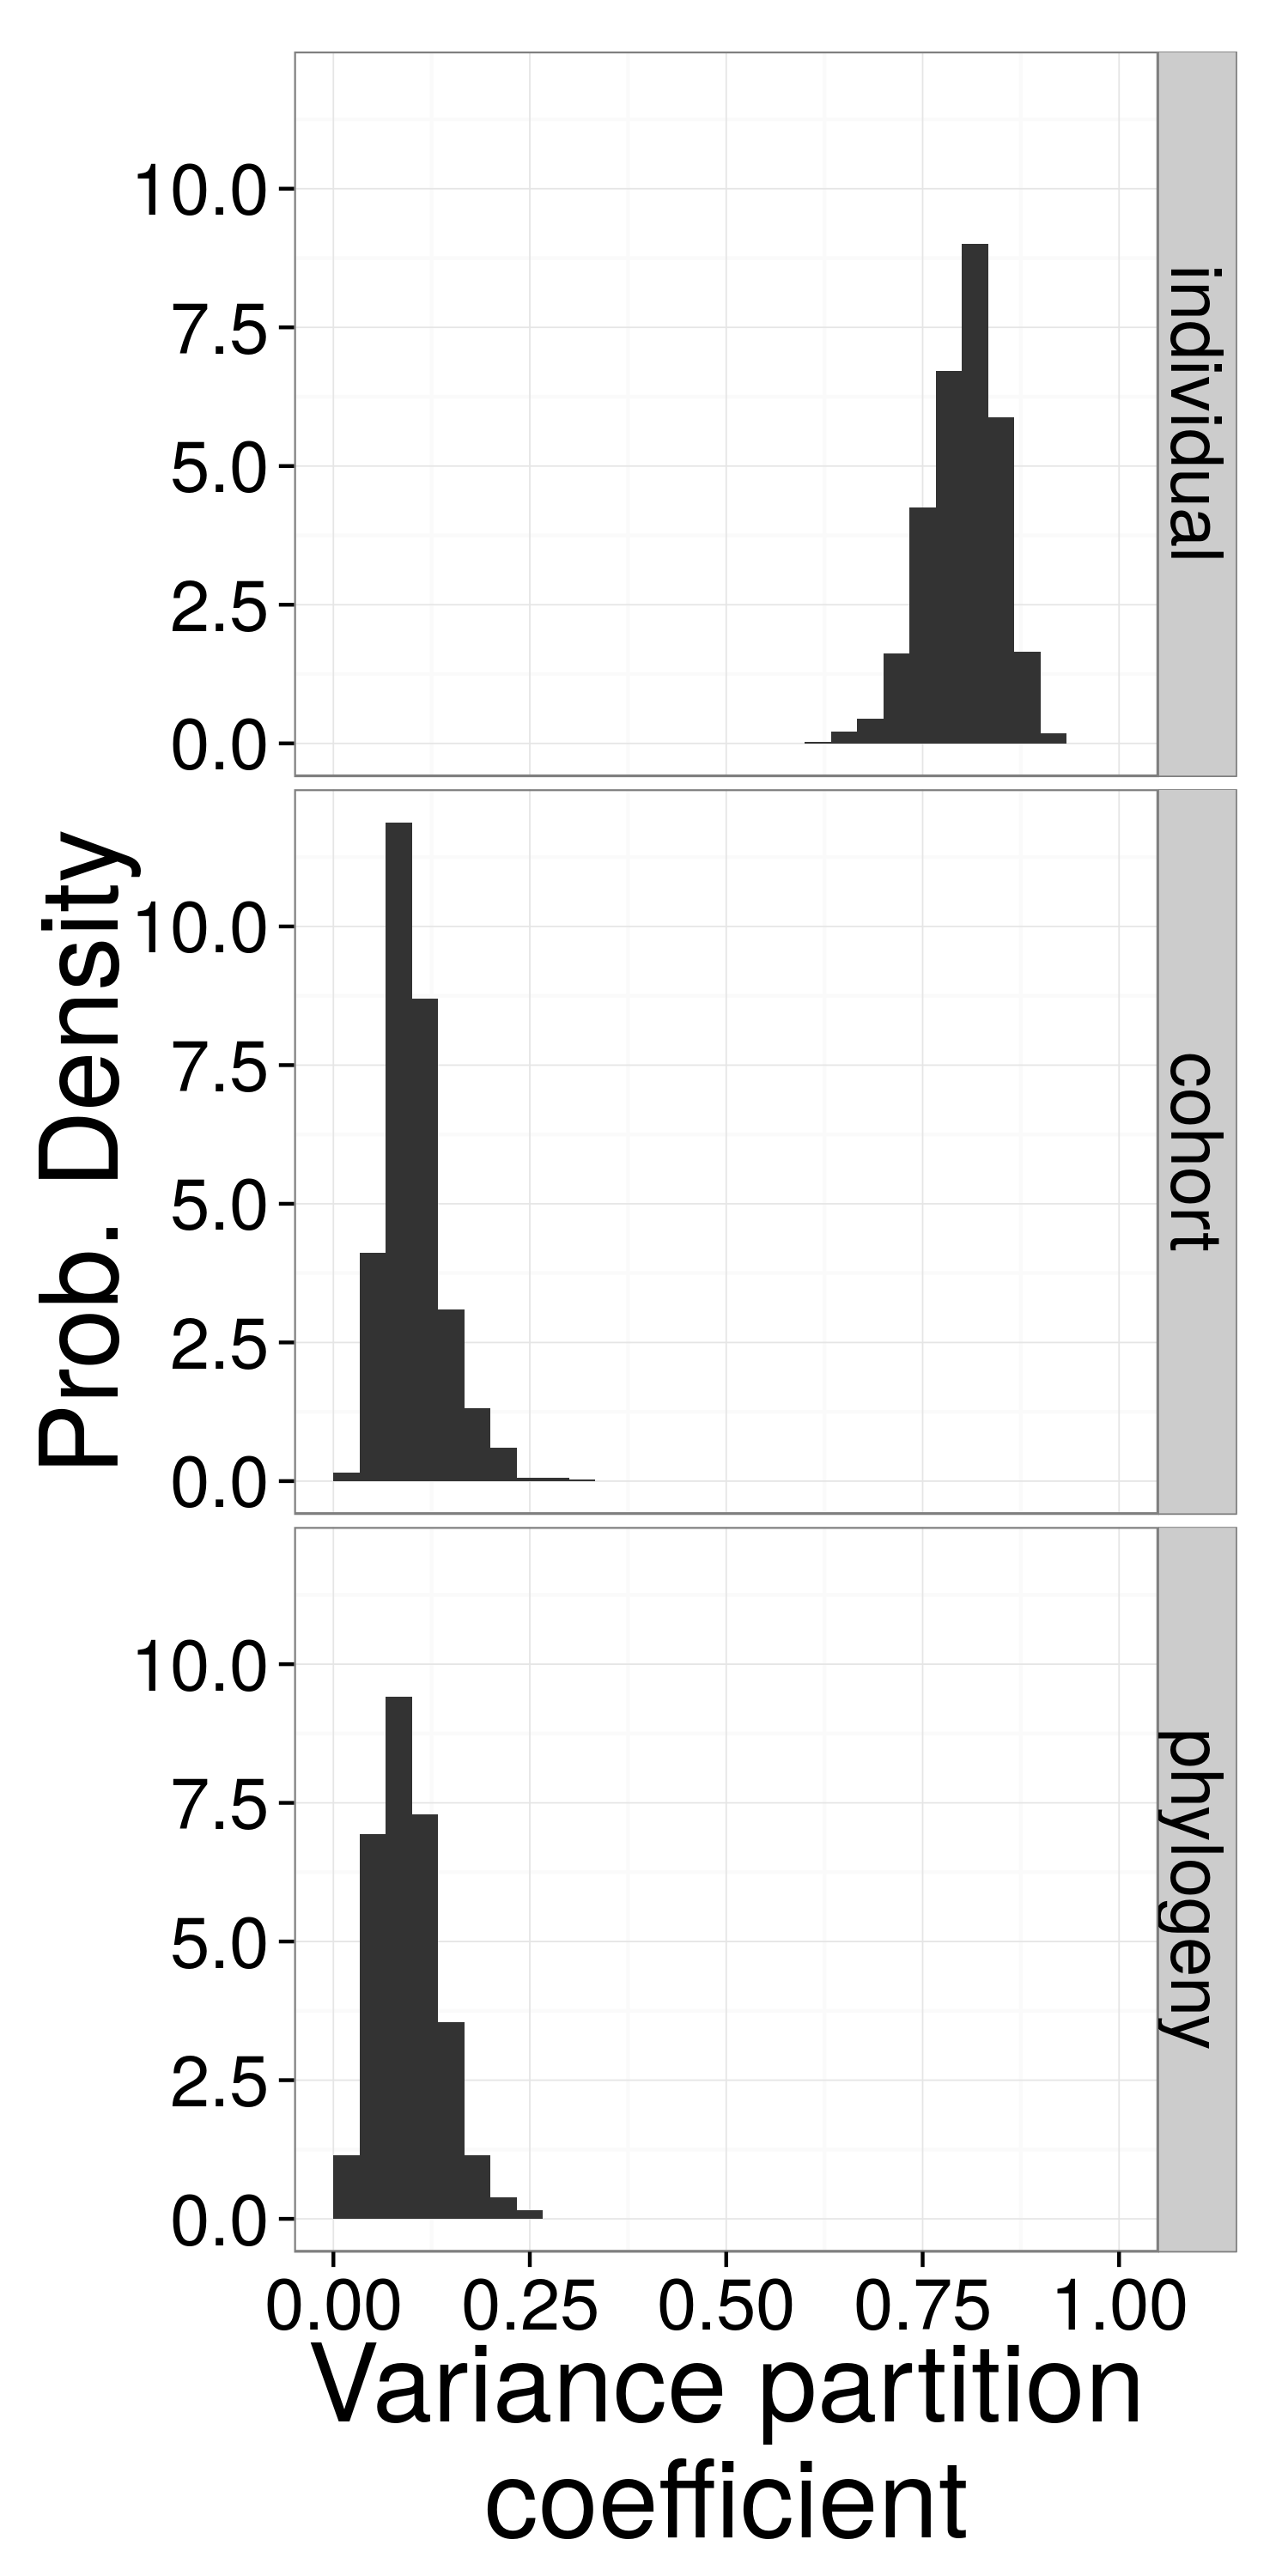
\includegraphics[width=\textwidth,height=0.8\textheight,keepaspectratio=true]{figure/variance_est}
    \end{column}
  \end{columns}
  
  \tiny{\attrib{Smits, \textit{Submitted}}}
  % covariate effects
  %   pairwise differences in indicator variables
  %   continuous covariates
  % VPC
\end{frame}

% *brachiopods*
\begin{frame}
  \frametitle{Study: brachiopod genus duration}

  \begin{alertblock}{Questions}
    \begin{itemize}
      \item How do the covariates of interest affect extinction risk?
        \begin{itemize}
          \item geographic range, environmental affinity, body size 
        \end{itemize}
      \item How do these effects vary between origination cohorts?
      \item How do changes in trait-based effects covary with changes in baseline extinction risk?
    \end{itemize}
  \end{alertblock}
\end{frame}

\begin{frame}
  \frametitle{Model of brachiopod genus survival}
 
  \begin{columns}
    \begin{column}{0.5\textwidth}
      \begin{align*}
        y_{i} &\sim \mathrm{Weibull}(\alpha, \sigma_{i}) \\
        \sigma_{i} &= \exp\left(\frac{-(\mathbf{X}_{i} \mathbf{B}_{j[i]})}{\alpha}\right) \\
        \mathbf{B}_{j} &\sim \mathrm{MVN}(\vec{\mu}, \mathbf{\Sigma}) \\
        \mathbf{\Sigma} &= \text{Diag}(\vec{\tau}) \mathbf{\Omega} \text{Diag}(\vec{\tau}) \\
        \alpha &\sim \mathrm{C^{+}}(2) \\
        \mu_{\kappa} &\sim \mathcal{N}(0, 5) \text{ for } \kappa \in 1:k \\
        \tau_{\kappa} &\sim \mathrm{C^{+}}(1) \text{ for } \kappa \in 1:k \\
        \mathbf{\Omega} &\sim \text{LKJ}(2).
      \end{align*}

      \bigskip

      \footnotesize{Unreadable. I know.}
    \end{column}
    \begin{column}{0.5\textwidth}
      Key details
      \begin{itemize}
        \item varying slopes, \\varying intercepts
        \item \(\mathbf{B}\): \(k \times J\) matrix of \(\beta\)-s
        \item \(\vec{\mu}\): hierarchical means of \(\beta\)-s
        \item \(\Sigma\): covariance matrix of (hierarchical) \(\beta\)-s
        \item \(\vec{\tau}\): vector of hierarchical scales (partial pooling)
        \item \(\Omega\): correlation matrix of (hierarchical) \(\beta\)-s
        \item model uncertainty in environmental affinity \\(not shown)
      \end{itemize}

    \end{column}
  \end{columns}
\end{frame}

\begin{frame}
  \frametitle{Results}
 
  \begin{columns}
    \begin{column}{0.5\textwidth}
      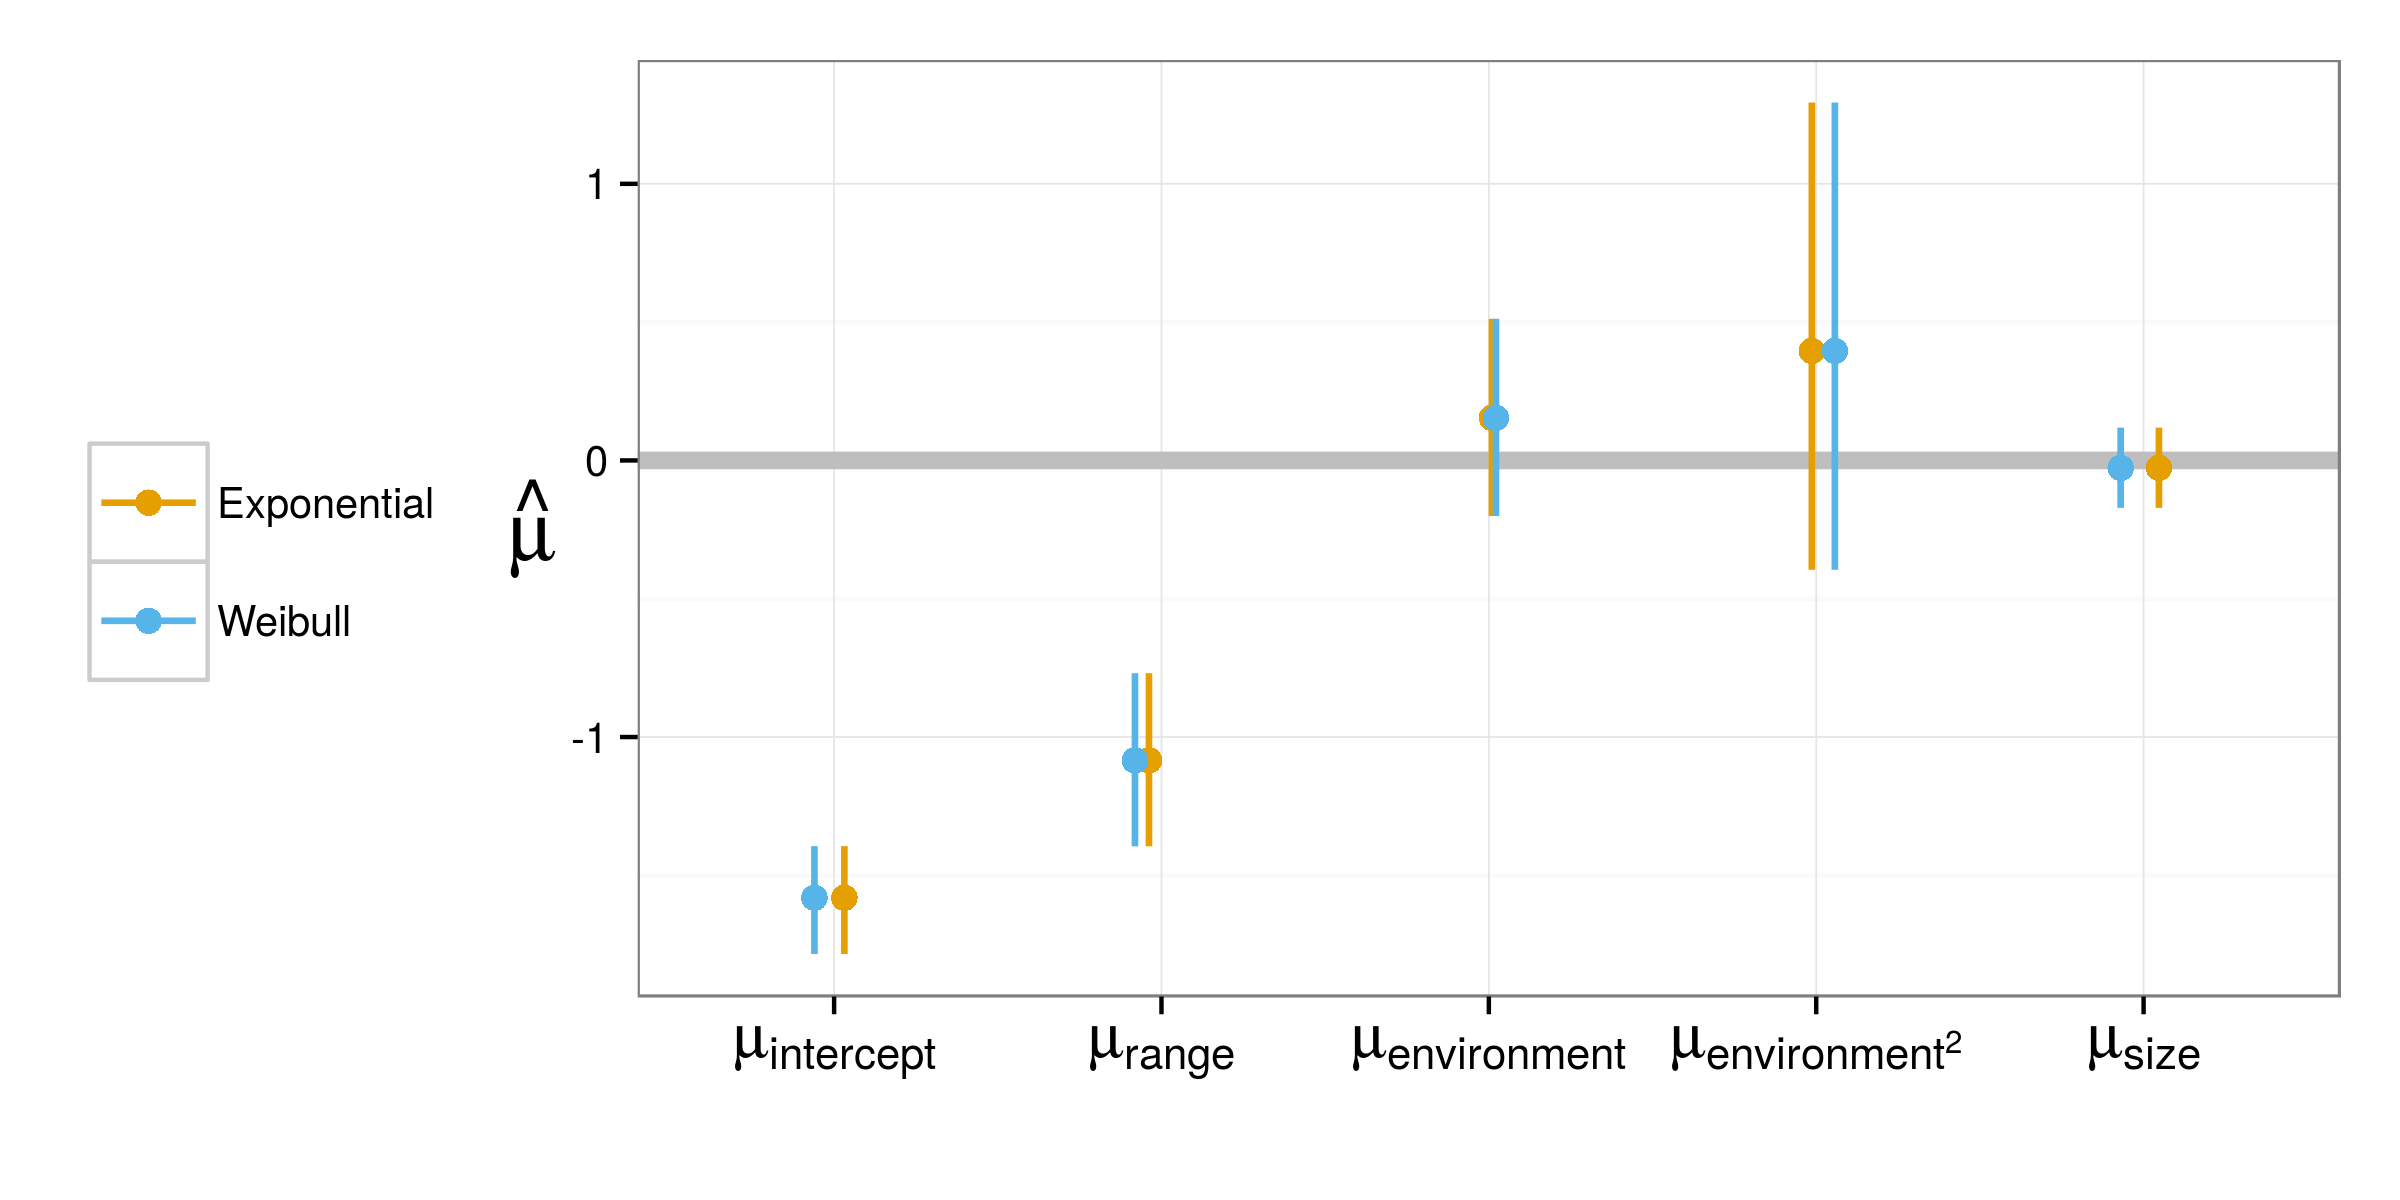
\includegraphics[width=\textwidth,keepaspectratio=true]{figure/coef_means}

      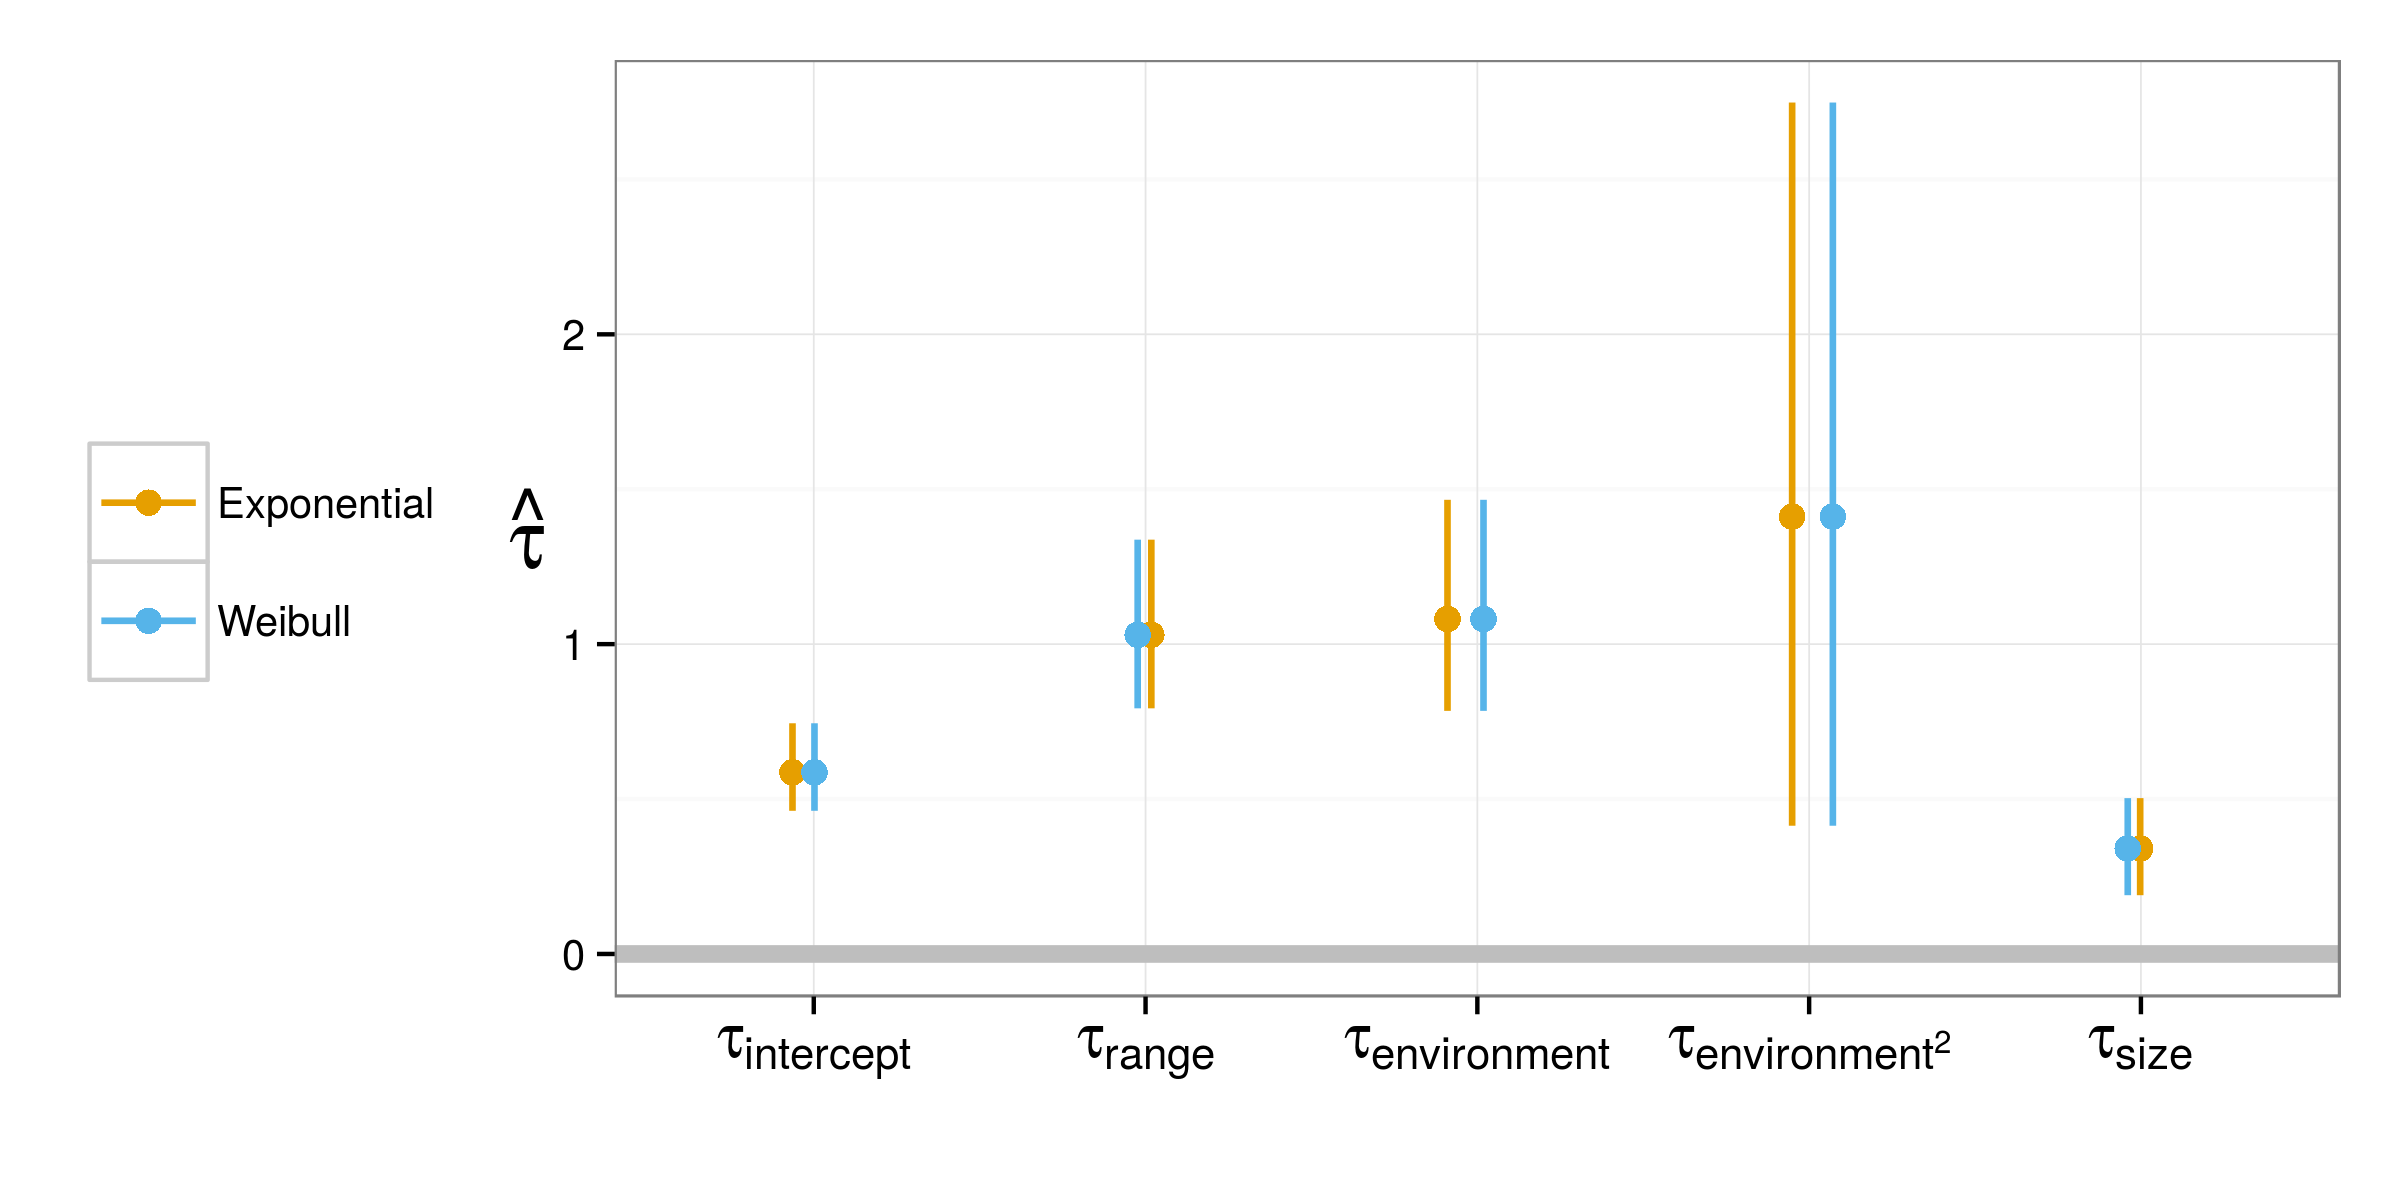
\includegraphics[width=\textwidth,keepaspectratio=true]{figure/coef_var}
    \end{column}
    \begin{column}{0.5\textwidth}
      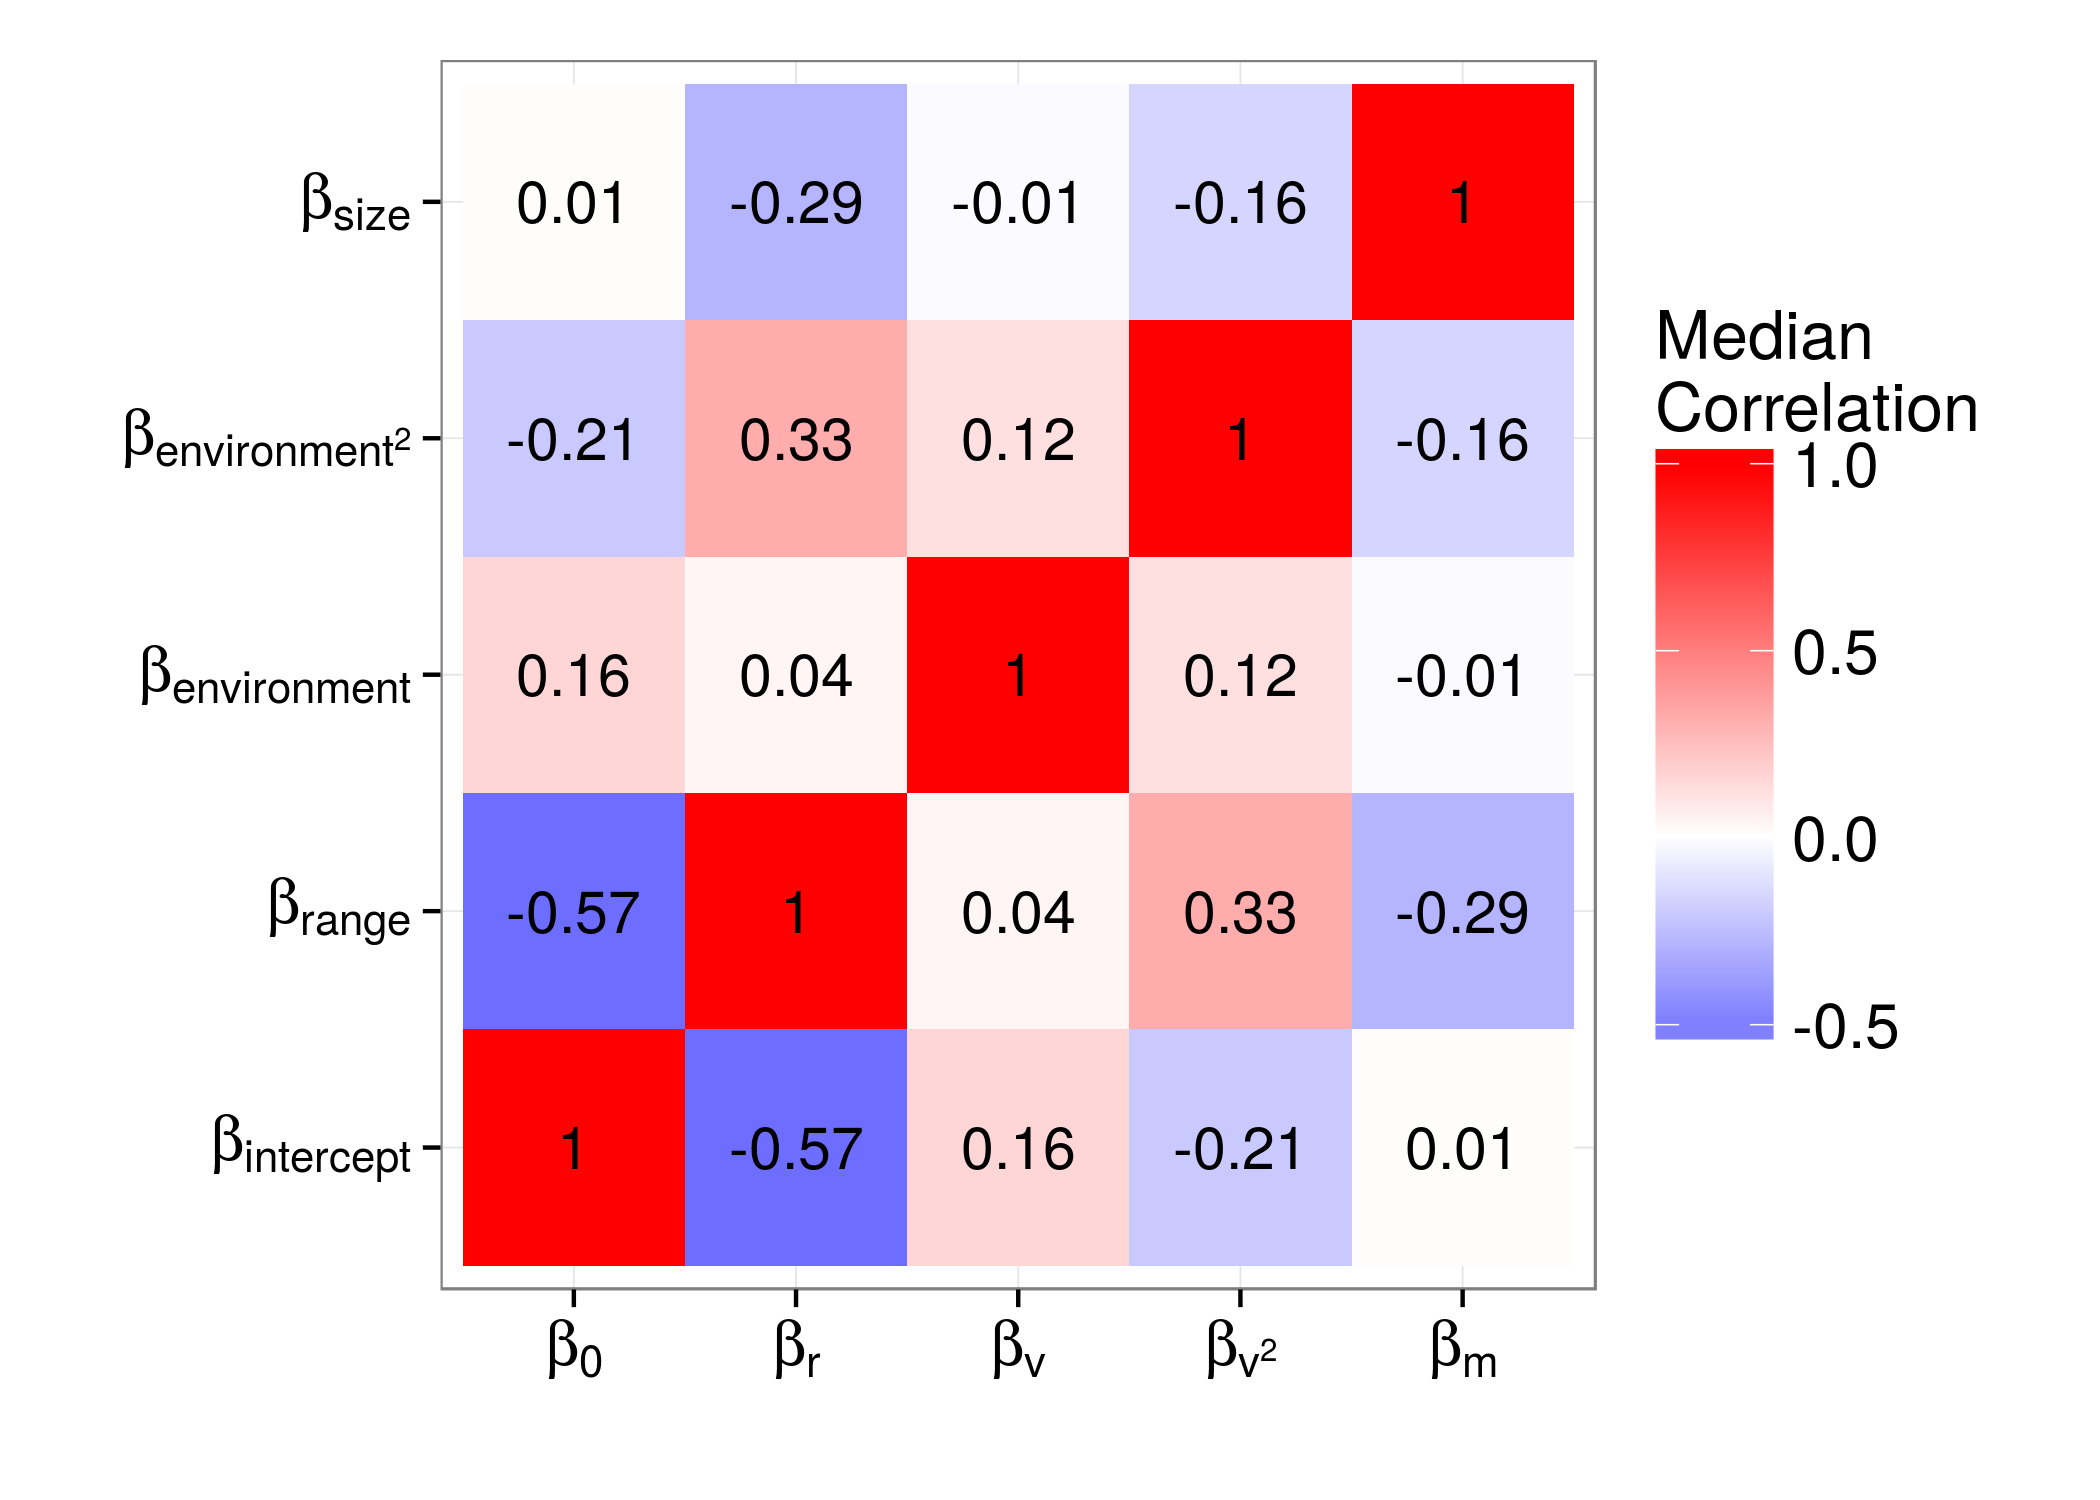
\includegraphics[width=\textwidth,keepaspectratio=true]{figure/wei_cor_heatmap}
    \end{column}
  \end{columns}
  
  \tiny{\attrib{Smits, \textit{In prep.}}}
\end{frame}

\begin{frame}
  \frametitle{Results}
  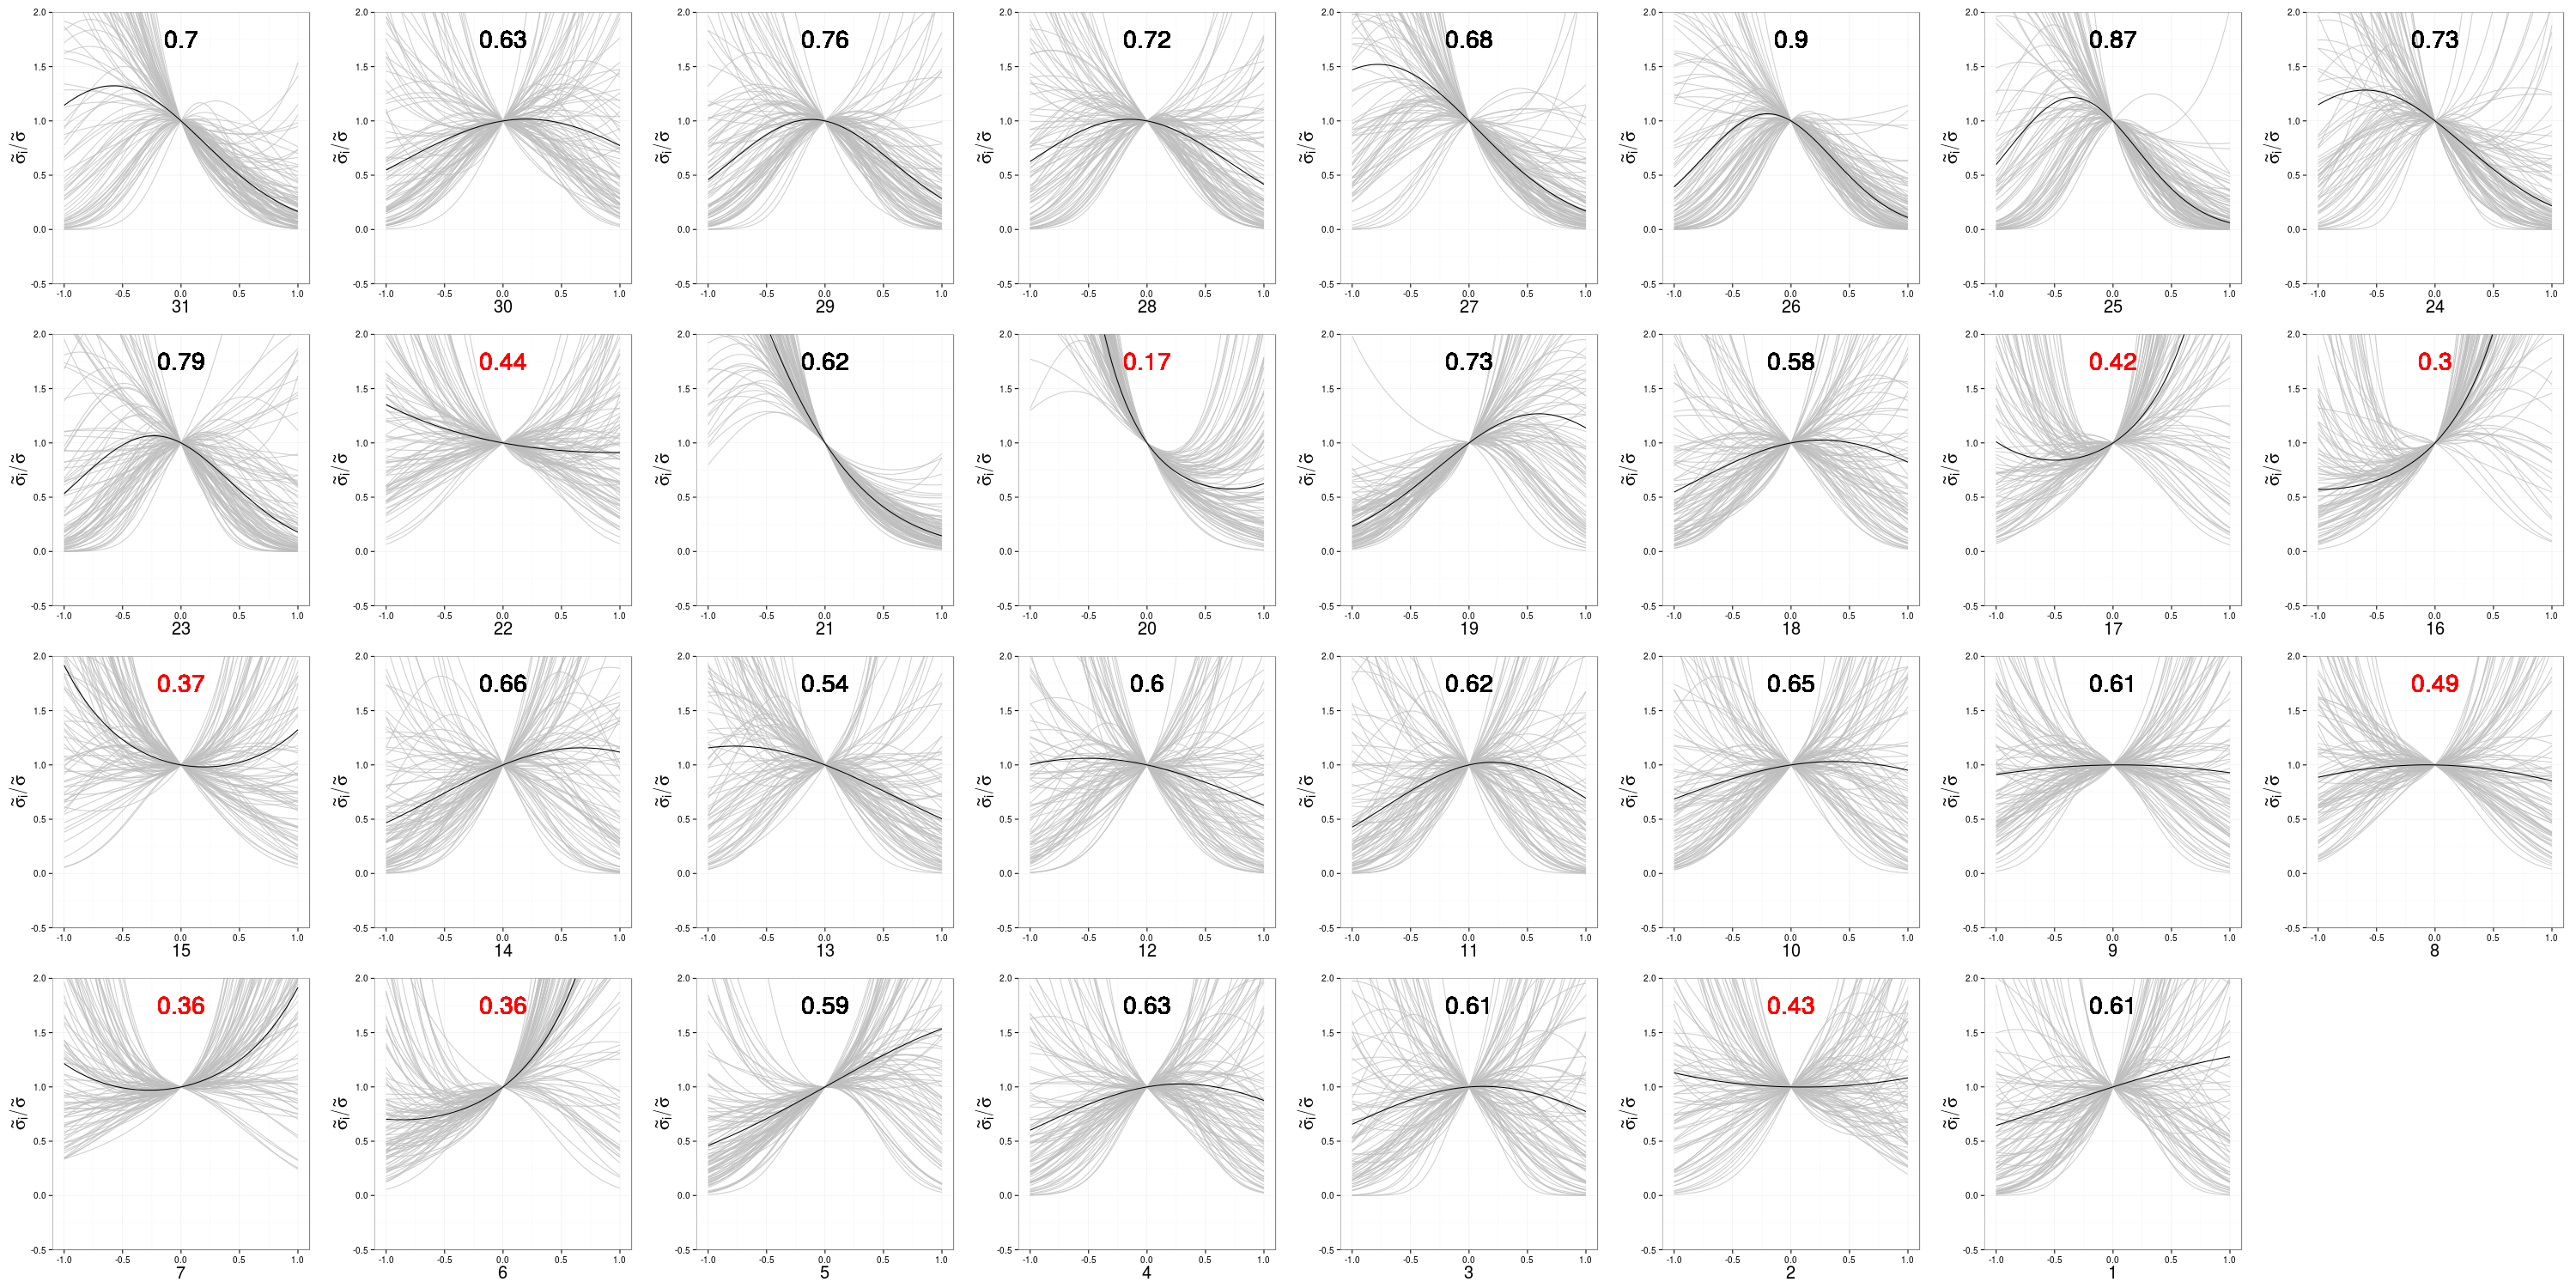
\includegraphics[width=\textwidth,keepaspectratio=true]{figure/cohort_quads}
  
  \tiny{\attrib{Smits, \textit{In prep.}}}
\end{frame}



\begin{frame}
  \frametitle{Summary}
  \begin{columns}
    \begin{column}{0.5\textwidth}
      \begin{center}
        \textbf{Mammals}

        \vspace{0.5cm}

        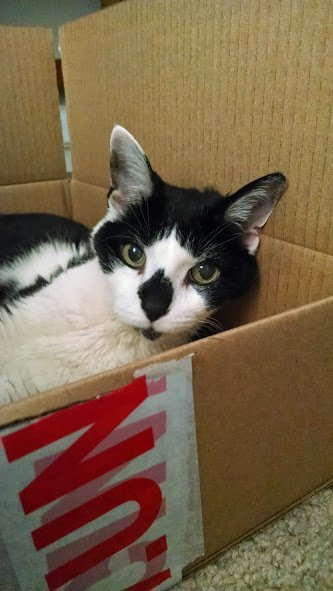
\includegraphics[height = 0.555\textheight, keepaspectratio = true]{figure/monty}
      \end{center}
    \end{column}
    \begin{column}{0.5\textwidth}
      \begin{center}
        \textbf{Brachiopods}
        
        \vspace{0.5cm}

        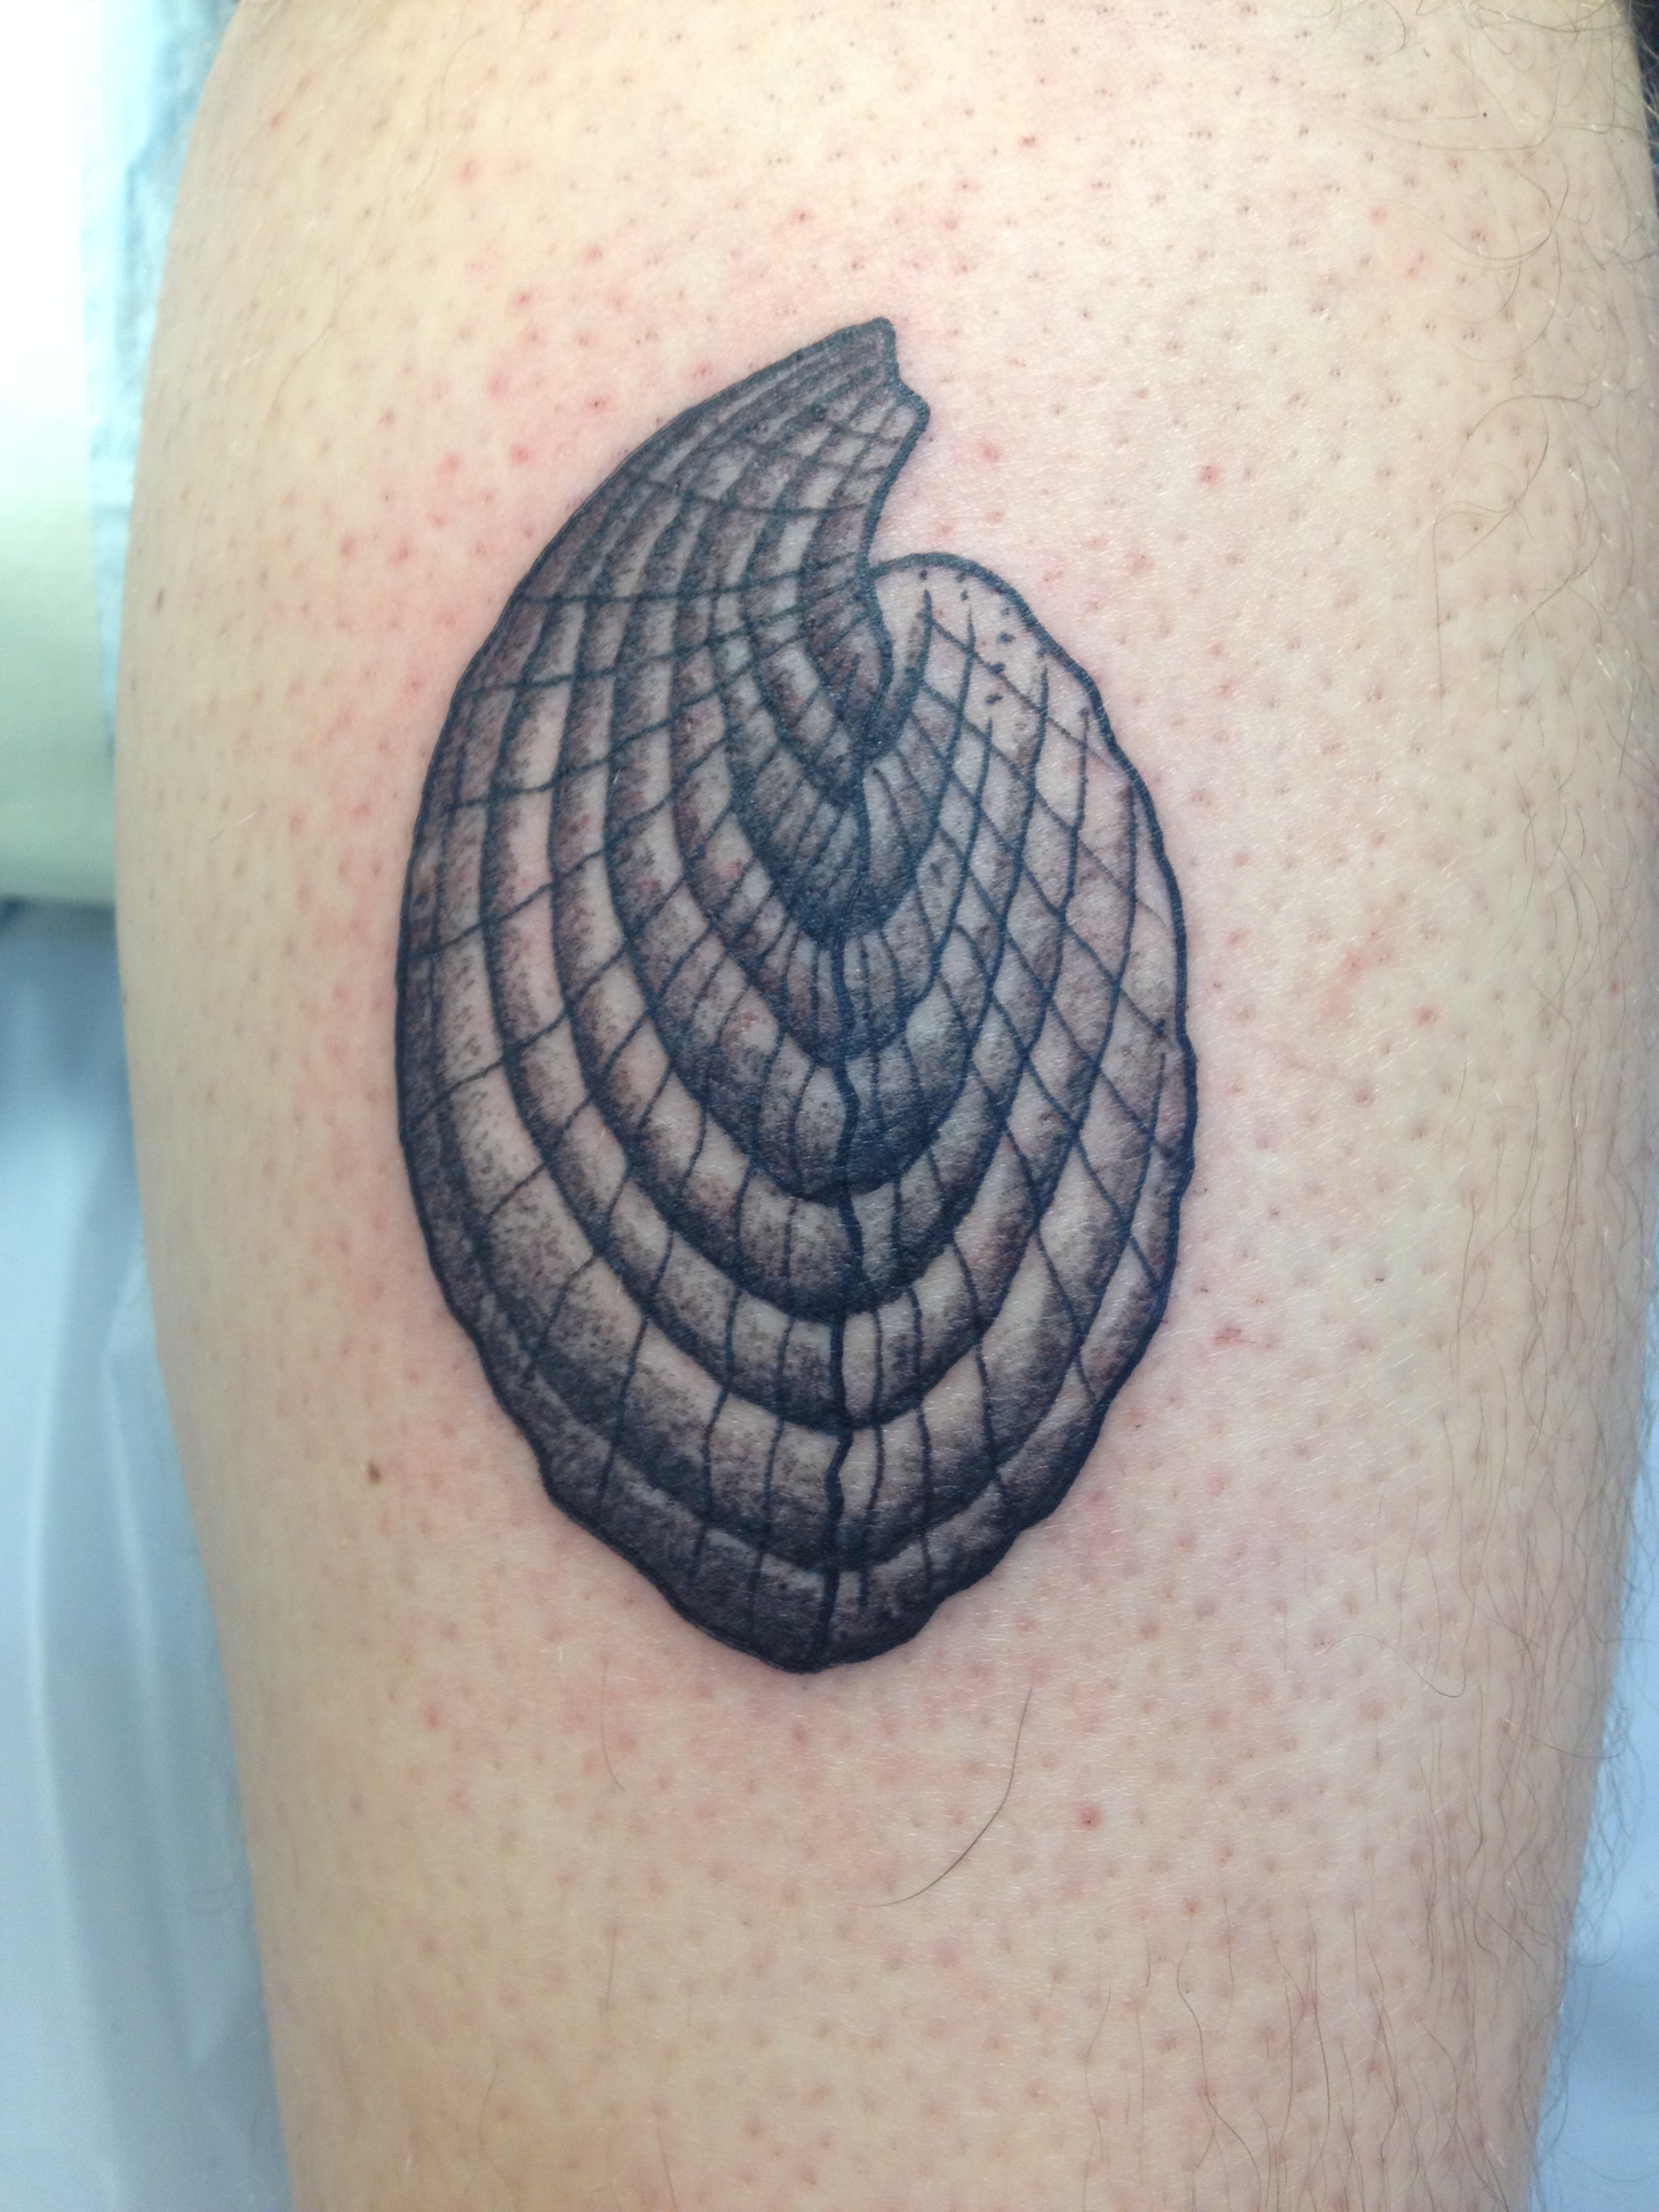
\includegraphics[height = 0.555\textheight, keepaspectratio = true]{figure/tattoo}
      \end{center}
    \end{column}
  \end{columns}
\end{frame}

% acknowledgements
%   committee
%   data sources
%   discussion
\begin{frame}
  \frametitle{Acknowledgements}
  \begin{columns}
    \begin{column}{0.5\textwidth}
      \begin{itemize}
        \item Advising
          \begin{itemize}
            \item Kenneth D. Angielczyk, Michael J. Foote, \\P. David Polly, \\Richard H. Ree
          \end{itemize}
        \item Angielczyk Lab
          \begin{itemize}
            \item David Grossnickle, \\Dallas Krentzel
          \end{itemize}
        \item Foote lab
          \begin{itemize}
            \item Marites Villarosa Garcia, \\Nadia Pierrehumbert, \\Kathleen Ritterbush
          \end{itemize}
      \end{itemize}
    \end{column}
    \begin{column}{0.5\textwidth}
      \begin{itemize}
        \item Other discussion
          \begin{itemize}
            \item Stewart Edie, \\Colin Kyle, \\Darcy Ross, \\Courtney Stepien
            \item John Alroy, \\David Bapst, \\Ben Frable, \\Graeme Lloyd, \\Carl Simpson, \\Graham Slater, \\Peter Wagner
          \end{itemize}
      \end{itemize}
    \end{column}
  \end{columns}
\end{frame}


\end{document}
